\section{A finite diagnostic of the heat-edge calculation}
\label{sec:diagnostic}

Figure~\ref{fig:edge-diagnostic} illustrates the three constants in the
positive exterior integral used in the proof of
Theorem~\ref{thm:heat-edge}. Write
\[
 I_{m,A}(s,c)=\frac1{\sqrt{4\pi s}}\int_0^\infty
 \cosh\!\left(m\operatorname{arcosh}(1+y/A)\right)
             e^{-(y-c)^2/(4s)}\,dy .
\]
At \(s=4\), the normalized saddle location, logarithmic amplitude,
and unit-coordinate logarithmic tilt tend respectively to
\(2^{5/3}\), \(3\,2^{-2/3}\), and \(2^{-4/3}\).
The computation evaluates the positive integral in logarithmic form;
it does not obtain a small residual by subtracting large Fourier
coefficients.

\begin{figure}[htbp]
 \centering
 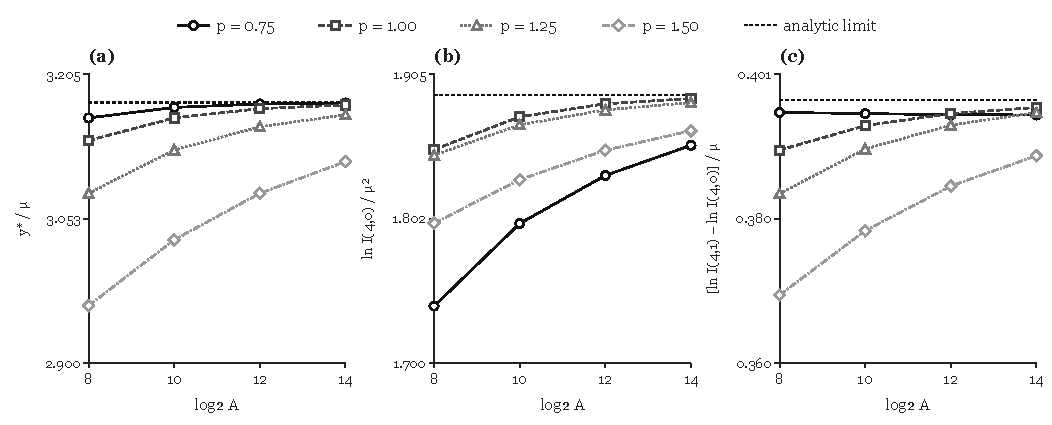
\includegraphics[width=\textwidth]{figures/heat-edge.pdf}
 \caption{Finite heat-edge diagnostic at \(s=4\).
 The four degree laws use \(m\) equal to the positive even integer
 nearest \(A^\sigma\), for \(\sigma=0.75,1,1.25,1.5\), and
 \(A=256,1024,4096,16384\).
 Panels (a)--(c) show the saddle location divided by \(\mu\),
 \(\log I_{m,A}(4,0)/\mu^2\), and
 \([\log I_{m,A}(4,1)-\log I_{m,A}(4,0)]/\mu\).
 Dashed horizontal lines are the three analytic limits. All quantities
 are dimensionless and natural logarithms are used in (b)--(c).
 Each panel has a separately enlarged vertical range. The
 \(\sigma=0.75\) tilt sequence moves slightly away from its limit on
 this finite grid; convergence is not asserted from these plotted
 values. The letter \(p\) in the figure legend denotes \(\sigma\)
 here, not the pressure or the scale parameter \(p_0\).}
 \label{fig:edge-diagnostic}
\end{figure}

The calculation uses deterministic IEEE-754 binary64
quadrature, with 40\,001 grid points for the fine calculation and
20\,001 for comparison, and a log-phase drop of 48 to truncate the
integration interval. The ancillary directory \texttt{anc/heat-edge/}
contains the plotting source, parameters, and all 16 data rows;
\texttt{plot.py --check} reproduces the numerical comparison report. The two-resolution and tail-truncation comparisons measure
stability of this finite calculation. They provide no error enclosure
for every degree and scale. The limiting assertions and the
Navier--Stokes conclusions are justified by the analytic proofs.

This figure illustrates the qualitative limits, not the
quantitative bounds or the second-kind extension. Exact algebra
checks are included in \texttt{anc/checks/}; neither is a continuum certificate.
